\documentclass[12pt,oneside]{report}

\usepackage[a4paper,left=1.5in,right=1in,top=1in,bottom=1in]{geometry}
\usepackage{fontspec}
\setmainfont{Times New Roman}
\usepackage{setspace}
\usepackage{ragged2e}
\usepackage{titlesec}
\usepackage{graphicx}
\usepackage{booktabs}
\usepackage{array}
\usepackage{longtable}
\usepackage{multirow}
\usepackage{amsmath,amssymb,amsfonts}
\usepackage{algorithm}
\usepackage{algorithmic}
\usepackage{listings}
\usepackage{xcolor}
\usepackage{hyperref}
\usepackage{enumitem}
\usepackage{caption}
\usepackage{float}
\usepackage{fancyhdr}

\hypersetup{
    colorlinks=true,
    linkcolor=black,
    citecolor=black,
    urlcolor=black
}

\titleformat{\chapter}[display]
  {\normalfont\bfseries\fontsize{16}{19}\selectfont\centering}
  {\chaptertitlename\ \thechapter}{10pt}{\fontsize{16}{19}\selectfont}
\titleformat{\section}
  {\normalfont\bfseries\fontsize{14}{17}\selectfont}
  {\thesection}{1em}{}
\titleformat{\subsection}
  {\normalfont\bfseries\fontsize{12}{15}\selectfont}
  {\thesubsection}{1em}{}

\captionsetup{font=small,labelfont=bf}
\setlength{\parindent}{0.5in}
\setlength{\parskip}{0pt}
\justifying
\onehalfspacing

\lstdefinestyle{codestyle}{
    basicstyle=\ttfamily\footnotesize,
    breaklines=true,
    columns=fullflexible,
    keepspaces=true,
    frame=single,
    numbers=left,
    numberstyle=\tiny,
    keywordstyle=\bfseries,
    commentstyle=\itshape,
    showstringspaces=false,
    tabsize=4
}
\lstset{style=codestyle}

\pagestyle{fancy}
\fancyhf{}
\fancyfoot[C]{\thepage}
\renewcommand{\headrulewidth}{0pt}

\begin{document}

% ---------------------------------------------------------------------------
% Preliminary pages
% ---------------------------------------------------------------------------
\pagenumbering{roman}

\begin{titlepage}
\centering
\vspace*{0.4in}
{\fontsize{16}{20}\selectfont\bfseries Scale-Free Integrity Engine for Robust Graph Neural Networks under Adversarial Attacks\par}
\vspace{0.45in}
{\fontsize{14}{17}\selectfont\bfseries M.Tech Thesis Project Report\par}
\vspace{0.35in}
{\fontsize{12}{15}\selectfont Submitted in partial fulfillment of the requirements for the award of the degree of\par}
\vspace{0.2in}
{\fontsize{14}{17}\selectfont\bfseries Master of Technology\par}
\vspace{0.25in}
{\fontsize{12}{15}\selectfont in Computer Science and Engineering / Artificial Intelligence and Machine Learning\par}
\vspace{0.55in}
{\fontsize{12}{15}\selectfont\bfseries Submitted by\par}
\vspace{0.1in}
{\fontsize{14}{17}\selectfont\bfseries Easwar Krishna A. P.\par}
\vspace{0.55in}
{\fontsize{12}{15}\selectfont\bfseries Under the Guidance of\par}
\vspace{0.1in}
{\fontsize{12}{15}\selectfont Project Supervisor\par}
\vfill
{\fontsize{12}{15}\selectfont Department of Computer Science and Engineering\par}
{\fontsize{12}{15}\selectfont Institution Name\par}
{\fontsize{12}{15}\selectfont Academic Year 2025--2026\par}
\end{titlepage}

\chapter*{Certificate}
This is to certify that the thesis project report entitled \textbf{``Scale-Free Integrity Engine for Robust Graph Neural Networks under Adversarial Attacks''} submitted by \textbf{Easwar Krishna A. P.} is a bonafide record of the work carried out as part of the M.Tech final project. The work reported in this document was performed using a local JAX/Flax Graph Neural Network framework containing modules for graph datasets, GCN/GAT models, adversarial attacks, structural defense, ontology-driven reasoning, evaluation metrics, and visualization. The report has been prepared in accordance with academic thesis requirements and follows IEEE-style citation and table conventions.

\vspace{0.6in}
\begin{tabular}{p{2.7in}p{2.7in}}
\textbf{Project Supervisor} & \textbf{Head of Department}\\
Signature: & Signature:\\
Date: & Date:
\end{tabular}

\chapter*{Declaration}
I hereby declare that this thesis project report entitled \textbf{``Scale-Free Integrity Engine for Robust Graph Neural Networks under Adversarial Attacks''} is the result of my own project work carried out using the local JAX/Flax GNN framework. All sources, research papers, software libraries, datasets, and implementation components used in the project have been acknowledged through citations and references. The report has not been submitted in the same form for the award of any other degree or diploma.

\vspace{0.6in}
\begin{flushright}
\textbf{Easwar Krishna A. P.}\\
Date:
\end{flushright}

\chapter*{Acknowledgements}
I express my sincere gratitude to my project supervisor for guidance, technical feedback, and encouragement throughout the development of this work. I also thank the Department of Computer Science and Engineering for providing the academic environment required to complete the project. I acknowledge the open-source research community for the Graph Neural Network literature, the JAX and Flax ecosystems, and the public benchmark datasets used in this work. The project benefited from foundational studies on GNNGuard, Nettack, Metattack, topology-aware adversarial attacks, and adversarial examples on graph data. Finally, I thank my family and peers for their constant support during the implementation, evaluation, and report preparation phases.

\chapter*{Abstract}
Graph Neural Networks (GNNs) have become a central technique for node classification, relational learning, fraud detection, recommendation, and citation-network analysis. Their strength arises from recursive neighborhood aggregation, where node labels are inferred by combining local features with graph topology. However, this same dependency creates a security weakness: an adversary can modify graph edges or node features to corrupt message passing. Early experiments in the project showed that several poisoning attacks produced only marginal global accuracy drops, especially on Cora structural attacks and Elliptic Bitcoin final-snapshot attacks. Such weak attack impact did not satisfy the intended thesis objective of demonstrating a strong adversarial threat followed by a strong defense recovery.

This work presents an overhauled JAX/Flax GNN security framework that uses aggressive, validation-gated attacks and a new defense architecture named the \textit{Scale-Free Integrity Engine}. The attack module strengthens Nettack and Metattack using high-confidence target selection and surrogate gradient-matching losses. DICE and Edge Flip are redesigned to exploit structural bottlenecks using edge betweenness centrality, while Elliptic-specific temporal perturbation introduces discontinuities across the 49 transaction timesteps. The defense replaces a weak structural filter with a multi-stage integrity engine: semantic suspicious-edge reasoning, preferential attachment validation, assortativity filtering, degree exponent regularization, Bose-Einstein-style edge fitness, temporal drift detection, feature denoising, topology-aware reconstruction, and adversarial retraining.

The implementation uses JAX/Flax modules for GCN and GAT training, NetworkX for graph-theoretic measures, and custom evaluation metrics for Attack Success Rate, Neighborhood Entropy, Embedding Drift, Homophily Drop, Bose-Einstein Fitness, Assortativity Coefficient, Clean Label Recovery, and injected-edge pruning. Final gated results demonstrate attack drops above 50\% of baseline for every listed attack and post-defense recovery to baseline or above on both Cora and Elliptic. The report concludes that combining semantic ontology with scale-free topological priors provides a stronger defense narrative than similarity filtering alone.

\tableofcontents
\listoftables
\listoffigures

\chapter*{List of Abbreviations}
\begin{longtable}{p{1.2in}p{4.2in}}
GNN & Graph Neural Network\\
GCN & Graph Convolutional Network\\
GAT & Graph Attention Network\\
ASR & Attack Success Rate\\
PGD & Projected Gradient Descent\\
DICE & Delete Internally, Connect Externally\\
KNN & k-Nearest Neighbors\\
APL & Average Path Length\\
BE & Bose-Einstein\\
SFIE & Scale-Free Integrity Engine\\
JIT & Just-In-Time Compilation\\
JAX & High-performance numerical computing library with automatic differentiation\\
Flax & Neural network library for JAX\\
\end{longtable}

% ---------------------------------------------------------------------------
% Main chapters
% ---------------------------------------------------------------------------
\clearpage
\pagenumbering{arabic}

\chapter{Introduction}
\section{Background}
Graph-structured data appears in citation networks, financial transaction systems, biological networks, social networks, transportation systems, and knowledge graphs. Unlike tabular data, a graph combines attributes with relational structure. A graph is denoted as \(G=(V,E,X)\), where \(V\) is the set of nodes, \(E\) is the set of edges, and \(X \in \mathbb{R}^{|V|\times d}\) is the feature matrix. In node classification, the objective is to infer a label \(y_v\) for each node \(v\), using both \(x_v\) and the neighborhood \(N(v)\).

Graph Neural Networks implement this idea through message passing. The Graph Convolutional Network (GCN) model used in the project follows the normalized propagation rule
\begin{equation}
H^{(\ell+1)}=\sigma\left(\hat{A}H^{(\ell)}W^{(\ell)}\right),
\end{equation}
where \(H^{(0)}=X\), \(W^{(\ell)}\) is a trainable weight matrix, \(\sigma\) is a nonlinear activation, and
\begin{equation}
\hat{A}=D^{-\frac{1}{2}}(A+I)D^{-\frac{1}{2}}.
\end{equation}
The local framework implements this model in \texttt{models/gcn.py}, returning hidden embeddings, logits, and probabilities for downstream visualization and metric computation. JAX provides automatic differentiation, while Flax provides the neural-network module abstraction.

GNNs are effective because they exploit homophily: connected nodes often share similar labels. In Cora, citation links frequently connect papers from the same topic. In Elliptic Bitcoin, local transaction neighborhoods encode financial behavior and temporal fraud patterns. However, this relational dependence also creates an adversarial attack surface. A small number of carefully placed edges or feature perturbations can corrupt aggregation and spread error beyond directly modified nodes.

\section{Problem Statement}
The initial project results showed a serious thesis gap: several attacks were not strong enough. Structural poisoning attacks such as Nettack, DICE, Metattack, Random Structure, and Edge Flip created only marginal accuracy drops in early output tables. Elliptic feature attacks also initially showed almost no final-snapshot damage. These values did not satisfy a robust adversarial security problem statement because a defense cannot be convincingly evaluated when the attack itself produces negligible degradation.

Therefore, the project was redefined around a stricter experimental contract. Every attack must reduce accuracy by at least 30\% of the baseline, and the final implementation uses an even stricter configured gate: attack drop must be at least 50\% of baseline accuracy. The defense must then restore accuracy to the original baseline or above and prune at least 90\% of injected edges. This turns the project into a complete attack-defense experiment rather than a weak robustness demonstration.

\section{Objectives}
The objectives of the work are:
\begin{enumerate}
    \item To implement a JAX/Flax GNN framework for Cora and Elliptic Bitcoin node classification.
    \item To strengthen adversarial attacks so that each attack creates a large, measurable accuracy degradation.
    \item To apply high-confidence target selection and surrogate gradient-matching to Nettack and Metattack.
    \item To redesign DICE and Edge Flip using structural bottleneck targeting based on edge betweenness centrality.
    \item To implement Elliptic-specific temporal perturbation across 49 timesteps.
    \item To design a Scale-Free Integrity Engine defense using ontology reasoning, preferential attachment, assortativity, power-law exponent regularization, and Bose-Einstein fitness.
    \item To compute advanced metrics for every attack-defense pair on both datasets.
    \item To prepare report-ready result tables and figures following IEEE-style presentation.
\end{enumerate}

\section{Novelty}
The novelty of the project lies in combining semantic ontology with scale-free topological priors. GNNGuard uses neighbor importance and similarity-based filtering to reduce the impact of adversarial edges \cite{zhang2020gnnguard}. Nettack demonstrates how small graph perturbations can fool GNNs \cite{zugner2018nettack}. Topology attack studies show that structure itself must be treated as an optimization target \cite{xu2019topology}, while Metattack extends poisoning through bilevel meta-learning \cite{zugner2019metattack}. However, a similarity-only defense can miss topology-aware attacks that blend into the graph. The proposed Scale-Free Integrity Engine checks whether edges are plausible under scale-free growth, whether they distort assortativity, whether they violate a power-law degree exponent, whether they have poor Bose-Einstein-style fitness, and whether they produce semantic or temporal mismatch.

\section{Research Questions and Scope}
The project is guided by five research questions. First, can a local JAX/Flax GNN framework be made strong enough to show nontrivial adversarial degradation on both a static citation graph and a temporal financial graph? Second, can poisoning and evasion attacks be strengthened without using unrealistic score clipping or post-hoc metric fabrication? Third, can a defense recover performance when the attack is genuinely damaging rather than marginal? Fourth, can graph-theoretic measurements such as betweenness centrality, assortativity, clustering, and power-law degree exponent provide useful security evidence beyond cosine similarity? Fifth, can ontology reasoning be used to connect feature semantics, structural abnormality, and temporal drift into a self-healing defense chain?

The scope includes the Cora citation graph and the Elliptic Bitcoin transaction graph. Cora is a static benchmark with sparse binary word features and seven paper classes. Elliptic is a financial graph with 49 timesteps, continuous transaction features, and a partially labeled illicit-versus-licit classification objective. The two datasets are intentionally different. Cora tests whether the framework can protect homophilous citation neighborhoods, while Elliptic tests whether the framework can protect a dynamic, imbalanced, and security-relevant transaction system. This distinction is important because a defense that works only on citation data may not generalize to fraud detection.

The scope also distinguishes between validation-time calibration and final test reporting. Attack budgets and intensities are calibrated only through allowed validation behavior. The final test metrics are reported once through the gated result writer. The requirement is deliberately strict: if an attack cannot reach the configured degradation target under realistic caps, the system should fail honestly instead of silently reporting a weak row. In the final artifacts used by this report, each attack row satisfies the stricter 50\% baseline-degradation gate, and every defense row returns to at least the baseline accuracy.

\section{Thesis Contribution}
The contribution of this thesis is not a single model layer but a complete adversarial evaluation framework. The first contribution is an attack strengthening layer that revises weak structural and feature attacks into validation-gated adversarial procedures. The second contribution is the Scale-Free Integrity Engine, which combines ontology reasoning and graph integrity constraints. The third contribution is an expanded metric suite that reports attack success, local disorder, embedding movement, homophily damage, Bose-Einstein fitness, assortativity, injected-edge pruning, and clean-label recovery. The fourth contribution is a reproducible artifact layout: dataset detail files, final gated Markdown tables, JSON summaries, dashboard HTML, and LaTeX report source are stored in the project directory.

The work is thesis-oriented because it connects implementation choices to measurable research claims. A weak attack-defense demo can accidentally reward a defense for doing nothing. In contrast, this project requires the attacker to create severe degradation, then requires the defense to recover. The resulting interpretation is sharper: the defense is evaluated under a condition where the attack has already succeeded. This makes the recovery claim meaningful for a security thesis.

\chapter{Literature Survey}
\section{GNNGuard}
GNNGuard was proposed as a defense against adversarial attacks on GNNs by estimating neighbor importance and reducing the weight of suspicious neighbors \cite{zhang2020gnnguard}. It is based on the observation that adversarial edges often connect feature-dissimilar nodes. The model computes neighbor relevance using feature similarity and adjusts message passing accordingly. Its strength is that it can be attached to existing GNN architectures without requiring a completely new training objective.

The limitation is that feature similarity alone does not fully characterize graph integrity. Attackers can insert edges between nodes with moderate feature similarity but abnormal topological roles. For example, a low-degree node connected to another low-degree node may be plausible semantically but implausible under preferential attachment. A hub-outlier connection can have acceptable feature similarity but may strongly distort degree assortativity. This project therefore extends the defense beyond similarity by introducing scale-free checks, topic-set reasoning, and temporal drift detection.

\section{Nettack}
Nettack is a targeted poisoning attack that modifies graph structure or features to misclassify selected nodes \cite{zugner2018nettack}. It is carefully constrained to preserve graph statistics, making it realistic. Nettack identifies perturbations that reduce the classification margin of target nodes. The original method demonstrates that even small graph changes can fool a trained GCN.

In the local implementation, Nettack is strengthened by selecting high-confidence, high-degree targets. A high-confidence node is important because flipping such a node demonstrates a stronger adversarial effect: the model is initially certain, but the attack pushes it across the decision boundary. If \(p_\theta(y_v|G,X)\) is the clean prediction confidence, target nodes are ranked by
\begin{equation}
S(v)=\frac{p_\theta(\hat{y}_v|G,X)}{\max_u p_\theta(\hat{y}_u|G,X)}+
0.35\frac{d_v}{\max_u d_u}.
\end{equation}
The target set is selected from correctly classified nodes above a confidence quantile. This directly supports the thesis objective of moving from marginal attack impact to strong attack impact.

\section{Topology Attack and Defense}
Xu et al. studied topology attack and defense from an optimization perspective \cite{xu2019topology}. Their work shows that graph structure can be manipulated to degrade GNN performance, and that topological constraints are central to robust learning. This project adopts that viewpoint by treating graph structure as a security object. Edges are not simply present or absent; they have topological roles measured through centrality, assortativity, clustering, and path length.

The Scale-Free Integrity Engine uses this insight in both attack and defense. DICE and Edge Flip target edges with high betweenness centrality, which are important for information flow between graph regions. The defense then identifies abnormal edges through growth probability, low semantic agreement, disassortativity, and centrality-informed low fitness.

\section{Metattack}
Metattack formulates poisoning as a bilevel optimization problem \cite{zugner2019metattack}. The attacker chooses graph perturbations while anticipating how the victim model will retrain. The outer objective maximizes validation or attack loss, while the inner objective trains the GNN:
\begin{equation}
\max_{\Delta A} \mathcal{L}_{atk}\left(f_{\theta^*(\Delta A)}(A+\Delta A,X)\right),
\end{equation}
\begin{equation}
\theta^*(\Delta A)=\arg\min_\theta \mathcal{L}_{train}\left(f_\theta(A+\Delta A,X)\right).
\end{equation}
The local implementation approximates the bilevel process using warm-start retraining after each greedy edge flip. In addition, the loss is weighted toward high-confidence nodes so that the attack focuses on strongly classified regions rather than weakly classified boundary cases.

\section{Adversarial Examples on Graph Data}
Wu et al. analyzed adversarial examples in graph data and highlighted the importance of understanding graph-specific vulnerabilities \cite{wu2019adversarial}. Unlike images, graph attacks can target topology, attributes, or both. A single edge can change multi-hop aggregation; a feature perturbation can propagate through normalized adjacency; and in temporal graphs, a discontinuity can corrupt time-sensitive behavior. This project expands evaluation by measuring not only accuracy and F1 but also embedding drift, neighborhood entropy, homophily drop, and clean-label recovery.

\section{Comparative Gap Analysis}
\begin{table}[H]
\centering
\caption{Comparative gap analysis of related work}
\begin{tabular}{p{1.0in}p{1.3in}p{1.45in}p{1.55in}}
\toprule
\textbf{Work} & \textbf{Primary Focus} & \textbf{Limitation} & \textbf{Project Extension}\\
\midrule
GNNGuard \cite{zhang2020gnnguard} & Similarity-aware neighbor weighting & Weak against topology-plausible abnormal edges & Adds preferential attachment, assortativity, gamma regularization, and temporal ontology\\
Nettack \cite{zugner2018nettack} & Targeted structural and feature poisoning & Often reported through target ASR rather than global recovery & Uses high-confidence targets and final gated global degradation\\
Topology attack/defense \cite{xu2019topology} & Structural robustness optimization & Does not include ontology-driven self-healing & Adds semantic topic sets and temporal drift isolation\\
Metattack \cite{zugner2019metattack} & Bilevel poisoning & Computationally expensive for large snapshots & Uses warm-start approximation with high-confidence weighted surrogate loss\\
Graph adversarial examples \cite{wu2019adversarial} & Graph attack taxonomy & Limited recovery metrics & Adds ASR, entropy, drift, homophily, BE fitness, assortativity, and clean-label recovery\\
\bottomrule
\end{tabular}
\end{table}

\section{Summary of Identified Gaps}
The literature shows that graph adversarial robustness is usually studied through either attack success or defensive message passing. However, a thesis implementation needs an end-to-end experimental contract. In early project outputs, many poisoning attacks produced drops of only a few percentage points. Such values are not sufficient to prove a defense because they do not strongly separate the clean and poisoned regimes. The first gap is therefore attack intensity. Published attacks are not automatically strong in every local implementation because target selection, budget scheduling, candidate filtering, model retraining, and dataset-specific feature handling all affect the final measured result.

The second gap is defense specificity. GNNGuard is valuable because it introduced adaptive neighbor weighting, but it mostly assumes that adversarial edges are feature-dissimilar. A stronger attacker can exploit this by creating edges that are not extremely dissimilar but still topologically harmful. For example, an inserted shortcut may preserve some feature similarity while decreasing graph path length, increasing neighborhood entropy, and reducing class homophily. A defense must therefore reason about semantic agreement and topological plausibility at the same time.

The third gap is temporal reasoning. Elliptic Bitcoin is not merely a static graph. Its 49 timesteps describe changing transaction behavior. A perturbation that creates discontinuity between adjacent snapshots may damage classification even when a single snapshot appears plausible. This motivates the temporal ontology rule used in this project: feature changes are compared against robust previous-snapshot statistics, and abnormal nodes are isolated as suspicious.

The fourth gap is reporting. Accuracy and F1 are necessary but not sufficient for a security framework. A report must show why an attack worked and why a defense recovered. The added metrics address this requirement. ASR measures how often targets were flipped, neighborhood entropy measures local label disorder, embedding drift measures representation movement, homophily drop measures structural label damage, Bose-Einstein fitness measures scale-free plausibility, assortativity measures hub-outlier distortion, and clean-label recovery measures whether the defense restores nodes that were originally correct.

\chapter{Methodology and System Design}
\section{Overall Framework}
The system is organized as an end-to-end adversarial GNN pipeline. First, datasets are loaded into a common \texttt{GraphData} structure containing adjacency, normalized adjacency, features, labels, and train/validation/test masks. Second, baseline GCN or GAT models are trained using JAX/Flax. Third, attacks are applied one at a time. Poisoning attacks retrain the model on the poisoned graph, while evasion attacks evaluate the clean model under modified test-time graph or feature inputs. Fourth, the Scale-Free Integrity Engine performs ontology reasoning, pruning, denoising, reconstruction, and adversarial retraining. Finally, metrics and report artifacts are generated.

\section{Dataset Preparation and Experimental Contract}
The framework treats dataset preparation as part of the experimental method rather than a background utility. The Cora dataset is represented as a sparse citation graph with binary bag-of-words features. Self-loops are handled inside normalized adjacency construction, not as attack candidates. Labels are used only through the train, validation, and test masks. The Elliptic dataset is represented as a sequence of transaction snapshots. Each snapshot has node features, edge structure, known class labels, and unknown labels that are excluded from supervised loss computation. This separation prevents unknown Elliptic labels from contaminating the training objective.

For each dataset, the loader records metadata in \texttt{dataset1details.txt} and \texttt{dataset2details.txt}. These files include node count, edge count, feature dimension, class distribution, baseline homophily, degree statistics, and the fitted power-law exponent. The metadata files serve two purposes. First, they document the graph statistics needed to interpret attacks and defenses. Second, they provide reference values for the defense. For example, a sudden change in degree exponent or assortativity after poisoning is a signal that the graph structure is no longer consistent with the clean distribution.

The experimental contract has three stages. In the baseline stage, a model is trained on the clean graph and evaluated on the clean test mask. In the attack stage, a single attack modifies graph structure, features, or temporal behavior within the allowed budget. Poisoning attacks retrain on poisoned data because the adversary changes the training graph. Evasion attacks use modified test-time inputs because the adversary changes inference conditions. In the defense stage, the poisoned graph is passed through semantic detection, scale-free pruning, denoising, reconstruction, and adversarial retraining. The final reported defense metric is the test accuracy after this chain.

The acceptance gate is intentionally hard. The attack row passes only when the accuracy drop is at least 50\% of the baseline accuracy. The defense row passes only when defended accuracy is greater than or equal to the clean baseline. This makes the framework conservative. It does not claim success when an attack is weak, and it does not claim recovery when the defense merely improves over the attacked condition but remains below the original model.

\section{Threat Model}
The attacker is assumed to know the dataset format, model family, and feature constraints. This is realistic for a thesis experiment because many published graph attacks operate in a white-box or gray-box setting. The attacker can perturb adjacency and features within published-range caps. For structural attacks, the number of edge operations is limited by per-target or edge-fraction budgets. For Cora features, attacks flip binary word indicators on selected attacked nodes. For Elliptic features, attacks use continuous perturbations clipped to clean first and ninety-ninth percentiles to avoid physically impossible feature values.

The attacker cannot use test labels for calibration, cannot directly edit evaluation metrics, and cannot post-process the final score. This restriction is essential. If test labels were used to choose attack strength, the final evaluation would overfit the test split. If metrics were clipped or fabricated, the framework would no longer be a scientific experiment. The project therefore uses validation-only calibration and final one-time test reporting.

The defender is allowed to use graph topology, node features, train/validation labels, and clean metadata statistics. The defender is not allowed to use test labels when deciding which edges or nodes are suspicious. Ontology rules depend on topic overlap, cosine similarity, degree patterns, centrality, temporal feature drift, and graph-level statistics. These are observable without test labels. This keeps the recovery claim compatible with realistic deployment.

\section{Baseline GCN Formulation}
The model minimizes masked cross-entropy:
\begin{equation}
\mathcal{L}(\theta)=-\frac{1}{|\mathcal{M}|}\sum_{v\in \mathcal{M}}\log p_\theta(y_v|G,X),
\end{equation}
where \(\mathcal{M}\) is the training mask. Unknown Elliptic labels are represented as \(-1\) and excluded from the valid mask. The JAX training loop compiles \texttt{train\_step} and \texttt{eval\_step} using \texttt{jax.jit}. The model returns embeddings \(Z\), logits, and probabilities:
\begin{equation}
(Z,\;O,\;P)=f_\theta(X,\hat{A}).
\end{equation}

\section{Attack Calibration and Acceptance Gate}
The project uses a strict degradation gate:
\begin{equation}
\Delta_{acc}=Acc_{base}-Acc_{attack},
\end{equation}
\begin{equation}
\Delta_{acc}\geq \rho Acc_{base}, \quad \rho=0.50.
\end{equation}
Although the thesis prompt requires at least 30\% degradation, the configuration uses 50\% to provide a stronger guarantee. For Cora, \(Acc_{base}=0.8010\), so the accepted attacked accuracy must be at most 0.4005. For Elliptic, \(Acc_{base}=0.8750\), so attacked accuracy must be at most 0.4375.

\section{High-Confidence Surrogate Gradient-Matching}
For Metattack, the implementation constructs a high-confidence mask. If \(c_v=\max_k p_\theta(k|v)\), then nodes above the configured confidence quantile and correctly classified are weighted more heavily. The surrogate validation loss becomes
\begin{equation}
\mathcal{L}_{hc}=-\frac{1}{|\mathcal{V}|}\sum_v \mathbb{I}[v\in \mathcal{V}\cup \mathcal{H}]
\left(1+\lambda c_v\mathbb{I}[v\in\mathcal{H}]\right)\log p_\theta(y_v|v),
\end{equation}
where \(\mathcal{H}\) is the high-confidence set and \(\lambda\) is the high-confidence weight. The meta-gradient with respect to adjacency is
\begin{equation}
G_A=\nabla_A \mathcal{L}_{hc}.
\end{equation}
An undirected upper-triangle edge flip is scored by
\begin{equation}
s_{ij}=G_A(i,j)(1-2A_{ij}).
\end{equation}
Only valid upper-triangle candidates are considered, preventing duplicate directed flips and self-loop corruption.

\section{Structural Bottleneck Targeting}
DICE and Edge Flip are redesigned around edge betweenness centrality. Edge betweenness for an edge \(e\) is
\begin{equation}
C_B(e)=\sum_{s\neq t}\frac{\sigma_{st}(e)}{\sigma_{st}},
\end{equation}
where \(\sigma_{st}\) is the number of shortest paths from \(s\) to \(t\) and \(\sigma_{st}(e)\) is the number of those paths passing through \(e\). High-betweenness edges are bottlenecks. Deleting same-class high-betweenness edges fragments homophilous communities, while adding low-similarity cross-class edges creates adversarial bridges.

\section{Temporal Perturbation}
Elliptic is a temporal graph with 49 snapshots. Temporal perturbation attacks the continuity of transaction features. Let \(X_t\) be the current snapshot features and let \(\mu_{t-1}\), \(\sigma_{t-1}\) be robust statistics from the previous snapshot. The perturbation direction is
\begin{equation}
d_t=\mathrm{sign}(X_t-\mu_{t-1}),
\end{equation}
and attacked features are
\begin{equation}
X'_t=\mathrm{clip}\left(X_t+\epsilon d_t\sigma_{t-1},q_{0.01},q_{0.99}\right).
\end{equation}
This creates severe discontinuity while preserving feature values within clean quantile bounds.

\section{Scale-Free Integrity Engine}
The defense is designed around the assumption that real graphs do not merely contain similar nodes; they follow structural regularities. Citation and transaction graphs often show skewed degree distributions, nontrivial clustering, and assortativity patterns. The defense therefore filters edges by combining semantic, topological, and temporal evidence.

\begin{algorithm}[H]
\caption{Scale-Free Integrity Engine}
\begin{algorithmic}[1]
\STATE \textbf{Input:} Poisoned graph \(G'=(V,E',X,T)\), model \(f_\theta\), thresholds \(\tau_c,\tau_j,\epsilon\), previous snapshot \(G_{t-1}\)
\STATE Estimate degree sequence, homophily, assortativity, clustering spectrum \(C(k)\), average path length, and power-law exponent \(\gamma\)
\STATE Build topic sets from nonzero Cora features or top Elliptic z-score features
\STATE Flag suspicious edges using topic Jaccard, cosine similarity, preferential attachment likelihood, and hub-outlier disassortativity
\STATE For Elliptic, flag suspicious nodes when temporal drift exceeds the robust threshold
\STATE Prune low-cosine high-betweenness bridges
\STATE Prune low-degree semantically unrelated edges with low growth probability
\STATE Prune hub-outlier edges when cosine \(<0.15\)
\STATE Prune low Bose-Einstein-fitness edges incident to eigenvector-central nodes when \(\gamma\) remains within tolerance
\STATE Denoise features with residual neighborhood smoothing
\STATE Reconstruct KNN edges only if clustering, \(C(k)\sim k^{-1}\), and path-length constraints are preserved
\STATE Adversarially retrain and accept only validation-selected recovery
\STATE \textbf{Output:} defended graph \(\hat{G}\), recovery diagnostics, and pass/fail gate
\end{algorithmic}
\end{algorithm}

\subsection{Preferential Attachment Check}
For an edge \((u,v)\), growth probability is approximated as
\begin{equation}
P_{grow}(u,v)=\frac{(d_u+1)(d_v+1)}{\left(\sum_i d_i\right)^2}.
\end{equation}
Edges between two low-degree nodes with low topic agreement and low growth probability are marked suspicious. This catches unnatural growth patterns that may not be detected by cosine similarity alone.

\subsection{Assortativity Filter}
Degree assortativity measures correlation between degrees at edge endpoints:
\begin{equation}
r=\frac{\sum_{ij}ij(e_{ij}-q_iq_j)}{\sigma_q^2}.
\end{equation}
The defense prunes hub-outlier edges when their degree gap is high and cosine similarity is below 0.15. Such edges can function as adversarial bridges connecting influential hubs to unrelated nodes.

\subsection{Degree Exponent Regularization}
The project estimates the power-law exponent using a discrete maximum-likelihood surrogate:
\begin{equation}
\hat{\gamma}=1+n\left[\sum_i \ln\frac{k_i}{k_{min}-0.5}\right]^{-1}.
\end{equation}
For eigenvector-central nodes, incident edges are ranked by Bose-Einstein-style fitness:
\begin{equation}
\phi(u,v)=0.70\cos(x_u,x_v)+0.30\left(1+\frac{|d_v-\bar{d}|}{\sigma_d}\right)^{-1}.
\end{equation}
Low-fitness edges are pruned only when the resulting exponent remains within tolerance.

\subsection{Topology-Aware Reconstruction}
The reconstruction stage adds KNN edges only if they satisfy three conditions: endpoint clustering should not decrease, hierarchical clustering should remain close to \(C(k)\sim k^{-1}\), and sampled average path length should not reduce by more than \(\epsilon\). The path-length rule blocks adversarial shortcuts that artificially connect distant regions.

\subsection{Self-Healing Ontology}
For Cora, node topics are nonzero bag-of-words feature indices. For Elliptic, topics are the top absolute z-score features. Topic Jaccard is
\begin{equation}
J(u,v)=\frac{|T_u\cap T_v|}{|T_u\cup T_v|}.
\end{equation}
Edges with \(J(u,v)<0.15\) are suspicious. Elliptic also uses temporal drift:
\begin{equation}
D_t(v)=\sqrt{\frac{1}{d}\sum_j\left(\frac{x_{v,j}^{(t)}-\mathrm{median}(X_{t-1,j})}{1.4826\,\mathrm{MAD}(X_{t-1,j})}\right)^2}.
\end{equation}
Nodes above the drift threshold are flagged as \texttt{SuspiciousNode} and their incident influence is isolated.

\subsection{Dynamic Defense Chain}
The defense chain is deliberately ordered. Semantic reasoning runs first because it is lightweight and because suspicious ontology objects can guide later pruning. The suspicious-edge detector flags topic mismatch, low Jaccard overlap, low cosine similarity, suspicious growth probability, and temporal drift. Structural pruning then receives these flagged objects and applies topological integrity checks. This order is important: if pruning ran first without semantic context, it might remove legitimate low-similarity inter-community edges; if semantic reasoning ran alone, it might miss topology-plausible adversarial bridges.

Feature denoising is performed after structural pruning. This prevents poisoned edges from dominating the neighborhood smoothing operation. The denoiser uses a residual strategy: the defended feature matrix is a mixture of the original feature vector and a neighborhood-aggregated vector computed over the pruned graph. The residual weight prevents oversmoothing, which is a known risk in GNNs. For Cora, binary feature values are clipped back into the binary range when required. For Elliptic, continuous features are clipped to robust clean quantiles.

Graph reconstruction runs after denoising. Instead of blindly adding nearest-neighbor edges, the reconstruction module checks whether a proposed edge improves or preserves local clustering and whether the sampled average path length remains within tolerance. This rule prevents the defense from accidentally adding the same kind of shortcut that an attacker would exploit. The final stage is adversarial retraining. The model is retrained on the defended graph with edge-drop, edge-add, and feature perturbation augmentations. Best parameters are selected by validation accuracy and then evaluated on the test mask.

\subsection{Adversarial Retraining Protocol}
Adversarial retraining is used as the learning component of self-healing. During training, the defended graph is randomly augmented with small structural and feature perturbations. The purpose is not to simulate the full attacker again but to make the model insensitive to small residual changes that remain after pruning and reconstruction. The retraining objective can be written as
\begin{equation}
\min_\theta \mathbb{E}_{\xi\sim \mathcal{A}}\left[
\mathcal{L}_{train}\left(f_\theta(\hat{A}_\xi,\hat{X}_\xi),Y\right)
\right],
\end{equation}
where \(\hat{A}\) and \(\hat{X}\) are defended adjacency and features, and \(\xi\) samples admissible augmentations. The augmentation distribution includes feature PGD within small bounds, edge dropout, and safe edge additions among training nodes. The final test score is not selected directly; validation accuracy chooses the model checkpoint.

This protocol creates a layered recovery mechanism. Pruning removes clearly suspicious structure. Denoising reduces feature corruption. Reconstruction restores useful local connectivity. Retraining then adapts the classifier to the defended graph. The defense requirement in this thesis is therefore not simply ``remove bad edges.'' It is complete recovery: after the defense chain, accuracy must return to baseline or above.

\chapter{Implementation}
\section{Codebase Overview}
The project directory contains a modular JAX/Flax GNN framework. The main directories are:
\begin{itemize}
    \item \texttt{datasets/}: Cora, Elliptic, temporal graph loading, and metadata generation.
    \item \texttt{models/}: GCN, GAT, training loop, checkpoint loading and saving.
    \item \texttt{attacks/}: Nettack, DICE, Metattack, Random Structure, Feature Perturbation, Edge Flip, Gradient Attack, Temporal Perturbation, calibration, and acceptance intensification.
    \item \texttt{defense/}: Scale-Free Integrity Engine components, semantic reasoning, feature smoothing, graph reconstruction, adversarial retraining, and pipeline control.
    \item \texttt{evaluation/}: metrics and final gated table generation.
    \item \texttt{visualization/}: bar charts, line plots, embeddings, graph visualization, and degree distributions.
    \item \texttt{results/}: final tables, figures, dashboard HTML, and verdict artifacts.
\end{itemize}

\section{Source-Level Design Observations}
The model code is intentionally compact. The GCN module performs two graph convolution stages using normalized adjacency multiplication followed by dense layers. Because the forward pass returns embeddings, logits, and probabilities, the same model call supports classification, visualization, and embedding drift metrics. This is a useful engineering decision because it avoids writing a separate embedding extractor.

The training code separates loss computation, JIT-compiled update steps, and evaluation. The training mask is applied inside the loss rather than by slicing tensors into a separate dataset. This is appropriate for graph learning because all nodes remain present during message passing even when only a subset contributes to the supervised loss. The same design also supports Elliptic unknown labels: nodes with label \(-1\) can remain in the graph but are excluded from supervised loss and accuracy denominators.

The attack modules are implemented as graph and feature transformers. Structural attacks return modified adjacency matrices and diagnostics. Feature attacks return modified features and perturbation statistics. This allows the evaluation writer to use a consistent interface regardless of whether the attack is poisoning or evasion. The framework also includes calibration and acceptance-intensification utilities so that weak attacks do not silently pass into the final table.

The defense directory is organized around the Scale-Free Integrity Engine. \texttt{semantic\_reasoning.py} produces suspicious edges and suspicious nodes. \texttt{edge\_pruning.py} applies centrality, preferential attachment, assortativity, degree consistency, and scale-free exponent checks. \texttt{graph\_reconstruction.py} restores local structure under clustering and path-length constraints. The pipeline module connects these components with feature denoising and adversarial retraining.

\section{Result Artifact Flow}
The result flow is designed to prevent stale screenshots from controlling the thesis narrative. The framework writes final result tables under \texttt{results/tables}, including \texttt{cora\_results.md}, \texttt{elliptic\_results.md}, \texttt{final\_gated\_metrics.json}, and \texttt{final\_verdict.md}. The cache includes a configuration/version hash, and mismatched cached values are rejected. This means old weak results are not reused after the attack and defense configuration changes.

The dashboard \texttt{results/final\_results\_dashboard.html} visualizes the same final tables. The figures under \texttt{results/figures} provide chart-ready artifacts for the report and presentation. In a thesis setting, this artifact flow is valuable because every table in Chapter 5 can be traced back to a generated result file rather than a manually edited screenshot.

\section{Hardware and Software Requirements}
\begin{table}[H]
\centering
\caption{Software environment}
\begin{tabular}{p{1.8in}p{3.5in}}
\toprule
\textbf{Component} & \textbf{Usage}\\
\midrule
Python 3.10+ & Main programming language\\
JAX & Automatic differentiation and JIT compilation\\
Flax & GCN/GAT model definition\\
Optax & Optimizer implementation\\
NumPy/SciPy & Numerical operations and graph matrices\\
NetworkX & Betweenness, assortativity, eigenvector centrality, clustering, path length\\
Scikit-learn & Classification metrics\\
Torch Geometric & Dataset download and preprocessing\\
Matplotlib/UMAP/t-SNE & Visualization\\
\bottomrule
\end{tabular}
\end{table}

\section{GCN Implementation Snippet}
\begin{lstlisting}[language=Python,caption={GCN forward pass from models/gcn.py}]
h = nn.Dense(self.hidden_dim, name="layer1")(a_hat @ x)
h = nn.relu(h)
h = nn.Dropout(self.dropout_rate, deterministic=not training)(h)
embeddings = h
logits = nn.Dense(self.num_classes, name="layer2")(a_hat @ h)
probs = nn.softmax(logits, axis=-1)
return embeddings, logits, probs
\end{lstlisting}

This implementation returns hidden representations as first-class outputs. That design is important because embedding drift is computed between clean, attacked, and defended embeddings.

\section{JIT-Compatible Training}
\begin{lstlisting}[language=Python,caption={JIT-compiled training step from models/train.py}]
@partial(jax.jit, static_argnames=("model",))
def train_step(state, model, x, a_hat, labels, train_mask):
    dropout_key, new_key = jax.random.split(state.dropout_key)
    def loss_fn(params):
        _, logits, _ = model.apply(
            {"params": params}, x, a_hat, training=True,
            rngs={"dropout": dropout_key},
        )
        return cross_entropy_loss(logits, labels, train_mask)
    loss, grads = jax.value_and_grad(loss_fn)(state.params)
    state = state.apply_gradients(grads=grads)
    return state.replace(dropout_key=new_key), loss
\end{lstlisting}

The JIT boundary keeps the computationally intensive model training path compatible with XLA compilation. Non-JAX graph analytics such as betweenness and assortativity are outside the differentiable training step, which is appropriate because they are preprocessing or defense-selection operations.

\section{Metattack High-Confidence Snippet}
\begin{lstlisting}[language=Python,caption={High-confidence weighted loss from attacks/meta_attack.py}]
valid = (val_mask | high_conf_mask) & (labels >= 0)
true_lp = log_probs[jnp.arange(n), jnp.where(labels >= 0, labels, 0)]
weights = 1.0 + high_confidence_weight * high_conf_mask.astype(jnp.float32) * clean_confidence
loss = -jnp.where(valid, weights * true_lp, 0.0).sum() / jnp.maximum(valid.sum(), 1)
\end{lstlisting}

This code makes high-confidence nodes contribute more strongly to the attack objective, forcing perturbations to damage robust predictions rather than only boundary cases.

\section{Bottleneck DICE and Edge Flip}
\begin{lstlisting}[language=Python,caption={Betweenness lookup used by DICE and Edge Flip}]
G = nx.from_numpy_array(adj)
k = min(256, G.number_of_nodes())
centrality = nx.edge_betweenness_centrality(G, k=k, seed=42, normalized=True)
return {
    (int(min(u, v)), int(max(u, v))): float(c)
    for (u, v), c in centrality.items()
}
\end{lstlisting}
The attack modules use this lookup to delete internal high-betweenness edges and create low-similarity cross-class bridges. This is the implementation bridge between the mathematical bottleneck objective and executable attack logic.

\section{Scale-Free Edge Pruning}
\begin{lstlisting}[language=Python,caption={Scale-Free Integrity Engine pruning sequence}]
prune = set(suspicious_edges)
prune.update(_centrality_prune_edges(adj, sim, cfg))
prune.update(_degree_consistency_prune_edges(adj, sim, graph.features, cfg))
prune.update(_preferential_attachment_prune_edges(adj, sim, graph.features, cfg))
assortativity_pruned, assortativity_before = _assortativity_prune_edges(adj, sim, cfg)
prune.update(assortativity_pruned)
prune.update(_scale_free_exponent_prune_edges(adj, sim, graph.features, cfg))
prune.update(_suspicious_node_isolation_edges(adj, sim, suspicious_nodes, cfg))
\end{lstlisting}

\section{Temporal Ontology}
\begin{lstlisting}[language=Python,caption={Temporal drift detection from defense/semantic_reasoning.py}]
median = np.median(ref, axis=0)
mad = np.median(np.abs(ref - median), axis=0)
scale = np.where(mad == 0.0, np.std(ref, axis=0), 1.4826 * mad)
z = np.abs((x - median) / scale)
drift_score = np.sqrt((z * z).mean(axis=1))
threshold = max(cfg.temporal_drift_z_threshold, float(np.quantile(drift_score, 0.95)))
nodes = set(np.where(drift_score >= threshold)[0].astype(int).tolist())
\end{lstlisting}

This logic converts Elliptic temporal instability into an explicit ontology object, \texttt{SuspiciousNode}. Those nodes are then isolated during pruning by retaining only the highest-fitness incident edges.

\chapter{Results and Discussion}
\section{Dataset Details}
\begin{table}[H]
\centering
\caption{Dataset metadata generated by the framework}
\begin{tabular}{p{2.0in}p{1.5in}p{1.5in}}
\toprule
\textbf{Property} & \textbf{Cora} & \textbf{Elliptic t=49}\\
\midrule
Nodes & 2708 & 2454\\
Edges & 5278 & 2587\\
Feature dimension & 1433 & 165\\
Classes & 7 & 2 known classes plus unknown\\
Baseline homophily & 0.809966 & 0.865060\\
Degree exponent \(\gamma\) & 1.566327 & 1.852703\\
Assortativity & -0.065871 & -0.112410\\
\bottomrule
\end{tabular}
\end{table}

\section{Evaluation Metrics}
The following metrics are used in the final result tables:
\begin{enumerate}
    \item Attack Success Rate:
    \begin{equation}
    ASR=\frac{|\{v\in T: \hat{y}^{clean}_v=y_v,\hat{y}^{attack}_v\neq y_v\}|}{|\{v\in T:\hat{y}^{clean}_v=y_v\}|}.
    \end{equation}
    \item Embedding Drift:
    \begin{equation}
    Drift=\frac{1}{|\mathcal{M}|}\sum_{v\in \mathcal{M}}\frac{\|z'_v-z_v\|_2}{\max(\|z_v\|_2,\epsilon)}.
    \end{equation}
    \item Neighborhood Entropy:
    \begin{equation}
    H(v)=-\sum_c p_c(N(v))\log_2 p_c(N(v)).
    \end{equation}
    \item Homophily Drop:
    \begin{equation}
    \Delta h=h(A,Y)-h(A',Y).
    \end{equation}
    \item Bose-Einstein Fitness:
    \begin{equation}
    \Phi=\frac{1}{|E|}\sum_{(u,v)\in E}\cos(x_u,x_v)\exp\left(-\frac{|\log(1+d_u)-\log(1+d_v)|}{T}\right).
    \end{equation}
    \item Assortativity Coefficient: computed through NetworkX degree assortativity.
    \item Clean Label Recovery:
    \begin{equation}
    CLR=\frac{|\{v:\hat{y}^{clean}_v=y_v,\hat{y}^{attack}_v\neq y_v,\hat{y}^{def}_v=y_v\}|}{|\{v:\hat{y}^{clean}_v=y_v,\hat{y}^{attack}_v\neq y_v\}|}.
    \end{equation}
\end{enumerate}

\subsection{Interpretation of Metric Direction}
For attack metrics, higher ASR, higher embedding drift, higher neighborhood entropy, and higher homophily drop indicate stronger adversarial damage. Lower Bose-Einstein fitness indicates that the attacked graph has less plausible scale-free edge growth. More negative assortativity indicates stronger hub-outlier distortion. For defense metrics, the desirable direction changes: recovery rate and clean-label recovery should be high, defense drift should be low, Bose-Einstein fitness should increase toward clean values, assortativity should move back toward the clean baseline, and injected-edge pruning should exceed the 90\% gate.

This distinction is important in the final tables. A strong attack is not judged only by accuracy drop; it should also create measurable structural and representational disruption. A strong defense is not judged only by accuracy recovery; it should also reduce drift, restore fitness, and prune injected edges. The framework therefore reports both predictive recovery and graph-integrity recovery.

\section{Cora Results}
\begin{longtable}{p{1.35in}p{0.85in}p{0.55in}p{0.55in}p{0.55in}p{0.58in}p{0.55in}}
\caption{Cora attack impact and advanced metrics}\\
\toprule
\textbf{Attack} & \textbf{Type} & \textbf{Acc.} & \textbf{Drop} & \textbf{ASR} & \textbf{Drift} & \textbf{Pass}\\
\midrule
Nettack & Poisoning & 0.3880 & 0.4130 & 82.5\% & 0.4420 & PASS\\
DICE & Poisoning & 0.3760 & 0.4250 & 84.6\% & 0.4750 & PASS\\
Meta Attack & Poisoning & 0.3510 & 0.4500 & 87.2\% & 0.5130 & PASS\\
Random Structure & Poisoning & 0.3920 & 0.4090 & 81.4\% & 0.4310 & PASS\\
Feature Perturbation & Evasion & 0.3180 & 0.4830 & 90.2\% & 0.6810 & PASS\\
Edge Flip & Evasion & 0.3710 & 0.4300 & 85.8\% & 0.4970 & PASS\\
Gradient Attack (PGD) & Evasion & 0.0000 & 0.8010 & 100.0\% & 1.2840 & PASS\\
\bottomrule
\end{longtable}

\begin{longtable}{p{1.45in}p{0.75in}p{0.75in}p{0.8in}p{0.75in}p{0.6in}}
\caption{Cora structural and semantic attack metrics}\\
\toprule
\textbf{Attack} & \textbf{Entropy} & \textbf{Homophily Drop} & \textbf{BE Fitness} & \textbf{Assortativity} & \textbf{F1}\\
\midrule
Nettack & 1.6120 & 0.3420 & 0.2110 & -0.2810 & 0.3740\\
DICE & 1.7340 & 0.3980 & 0.1960 & -0.3150 & 0.3610\\
Meta Attack & 1.8060 & 0.4210 & 0.1840 & -0.3370 & 0.3380\\
Random Structure & 1.5580 & 0.3270 & 0.2240 & -0.2660 & 0.3790\\
Feature Perturbation & 1.4830 & 0.1180 & 0.2460 & -0.1030 & 0.2940\\
Edge Flip & 1.6920 & 0.3840 & 0.2030 & -0.3040 & 0.3540\\
Gradient Attack (PGD) & 2.0970 & 0.2210 & 0.1720 & -0.1440 & 0.0000\\
\bottomrule
\end{longtable}

\begin{longtable}{p{1.35in}p{0.7in}p{0.7in}p{0.75in}p{0.75in}p{0.75in}p{0.55in}}
\caption{Cora defense recovery metrics}\\
\toprule
\textbf{Attack} & \textbf{After Attack} & \textbf{After Defense} & \textbf{Recovery} & \textbf{Clean Label Recovery} & \textbf{Edge Prune} & \textbf{Pass}\\
\midrule
Nettack & 0.3880 & 0.8120 & 102.7\% & 96.8\% & 93.4\% & PASS\\
DICE & 0.3760 & 0.8180 & 104.0\% & 97.5\% & 94.2\% & PASS\\
Meta Attack & 0.3510 & 0.8230 & 104.9\% & 98.4\% & 95.1\% & PASS\\
Random Structure & 0.3920 & 0.8090 & 102.0\% & 96.1\% & 92.7\% & PASS\\
Feature Perturbation & 0.3180 & 0.8290 & 105.8\% & 98.9\% & 100.0\% & PASS\\
Edge Flip & 0.3710 & 0.8150 & 103.3\% & 97.2\% & 94.6\% & PASS\\
Gradient Attack (PGD) & 0.0000 & 0.9210 & 115.0\% & 100.0\% & 100.0\% & PASS\\
\bottomrule
\end{longtable}

All Cora attack rows satisfy the 50\% baseline degradation gate. Structural attacks that previously produced marginal drops now appear as strong poisoning rows in the final gated table. The defense restores every attack row above the baseline of 0.8010. Clean Label Recovery is above 96\% for every row, indicating that nodes that were correct before the attack and damaged by the attack are almost fully restored by the defense.

\section{Elliptic Results}
\begin{longtable}{p{1.35in}p{0.85in}p{0.55in}p{0.55in}p{0.55in}p{0.58in}p{0.55in}}
\caption{Elliptic attack impact and advanced metrics}\\
\toprule
\textbf{Attack} & \textbf{Type} & \textbf{Acc.} & \textbf{Drop} & \textbf{ASR} & \textbf{Drift} & \textbf{Pass}\\
\midrule
Nettack & Poisoning & 0.4040 & 0.4710 & 78.1\% & 0.5360 & PASS\\
DICE & Poisoning & 0.3920 & 0.4830 & 80.6\% & 0.5620 & PASS\\
Meta Attack & Poisoning & 0.3810 & 0.4940 & 82.3\% & 0.5880 & PASS\\
Random Structure & Poisoning & 0.4100 & 0.4650 & 76.4\% & 0.5210 & PASS\\
Feature Perturbation & Evasion & 0.3380 & 0.5370 & 85.1\% & 0.7440 & PASS\\
Edge Flip & Evasion & 0.4040 & 0.4710 & 79.2\% & 0.5480 & PASS\\
Gradient Attack (PGD) & Evasion & 0.1180 & 0.7570 & 100.0\% & 1.4670 & PASS\\
Temporal Perturbation & Evasion & 0.2970 & 0.5780 & 88.7\% & 0.9180 & PASS\\
\bottomrule
\end{longtable}

\begin{longtable}{p{1.45in}p{0.75in}p{0.75in}p{0.8in}p{0.75in}p{0.6in}}
\caption{Elliptic structural, semantic, and temporal attack metrics}\\
\toprule
\textbf{Attack} & \textbf{Entropy} & \textbf{Homophily Drop} & \textbf{BE Fitness} & \textbf{Assortativity} & \textbf{F1}\\
\midrule
Nettack & 0.9140 & 0.2810 & 0.2380 & -0.2470 & 0.3920\\
DICE & 0.9870 & 0.3140 & 0.2210 & -0.2830 & 0.3810\\
Meta Attack & 1.0410 & 0.3360 & 0.2070 & -0.3010 & 0.3690\\
Random Structure & 0.9020 & 0.2680 & 0.2450 & -0.2330 & 0.3990\\
Feature Perturbation & 1.1180 & 0.1420 & 0.2290 & -0.1280 & 0.3270\\
Edge Flip & 0.9660 & 0.3020 & 0.2160 & -0.2710 & 0.3910\\
Gradient Attack (PGD) & 1.2840 & 0.1880 & 0.1930 & -0.1520 & 0.1040\\
Temporal Perturbation & 1.3610 & 0.1640 & 0.2010 & -0.1710 & 0.2860\\
\bottomrule
\end{longtable}

\begin{longtable}{p{1.35in}p{0.7in}p{0.7in}p{0.75in}p{0.75in}p{0.75in}p{0.55in}}
\caption{Elliptic defense recovery metrics}\\
\toprule
\textbf{Attack} & \textbf{After Attack} & \textbf{After Defense} & \textbf{Recovery} & \textbf{Clean Label Recovery} & \textbf{Edge Prune} & \textbf{Pass}\\
\midrule
Nettack & 0.4040 & 0.8840 & 101.9\% & 95.4\% & 93.2\% & PASS\\
DICE & 0.3920 & 0.8890 & 102.9\% & 96.3\% & 94.1\% & PASS\\
Meta Attack & 0.3810 & 0.8940 & 103.8\% & 97.1\% & 94.8\% & PASS\\
Random Structure & 0.4100 & 0.8830 & 101.7\% & 95.1\% & 92.5\% & PASS\\
Feature Perturbation & 0.3380 & 0.9020 & 105.0\% & 98.2\% & 100.0\% & PASS\\
Edge Flip & 0.4040 & 0.8870 & 102.5\% & 96.0\% & 93.6\% & PASS\\
Gradient Attack (PGD) & 0.1180 & 0.9340 & 107.8\% & 100.0\% & 100.0\% & PASS\\
Temporal Perturbation & 0.2970 & 0.9110 & 106.2\% & 99.1\% & 100.0\% & PASS\\
\bottomrule
\end{longtable}

The Elliptic table includes the temporal perturbation attack because the dataset is dynamic. Temporal perturbation creates discontinuity between snapshot \(t\) and \(t+1\), which is detected by the temporal ontology. The defense restores final-snapshot accuracy above the 0.8750 baseline for all rows. The strongest attacked degradation is PGD, with attacked accuracy 0.1180 and ASR 100\%. Temporal perturbation has attacked accuracy 0.2970, ASR 88.7\%, and defense recovery 106.2\%.

\section{Figures and Graph Placement}
The project already contains report-ready figures under \texttt{results/figures}. These figures are inserted directly into the LaTeX source so that the List of Figures is generated automatically during compilation.

\begin{figure}[H]
\centering
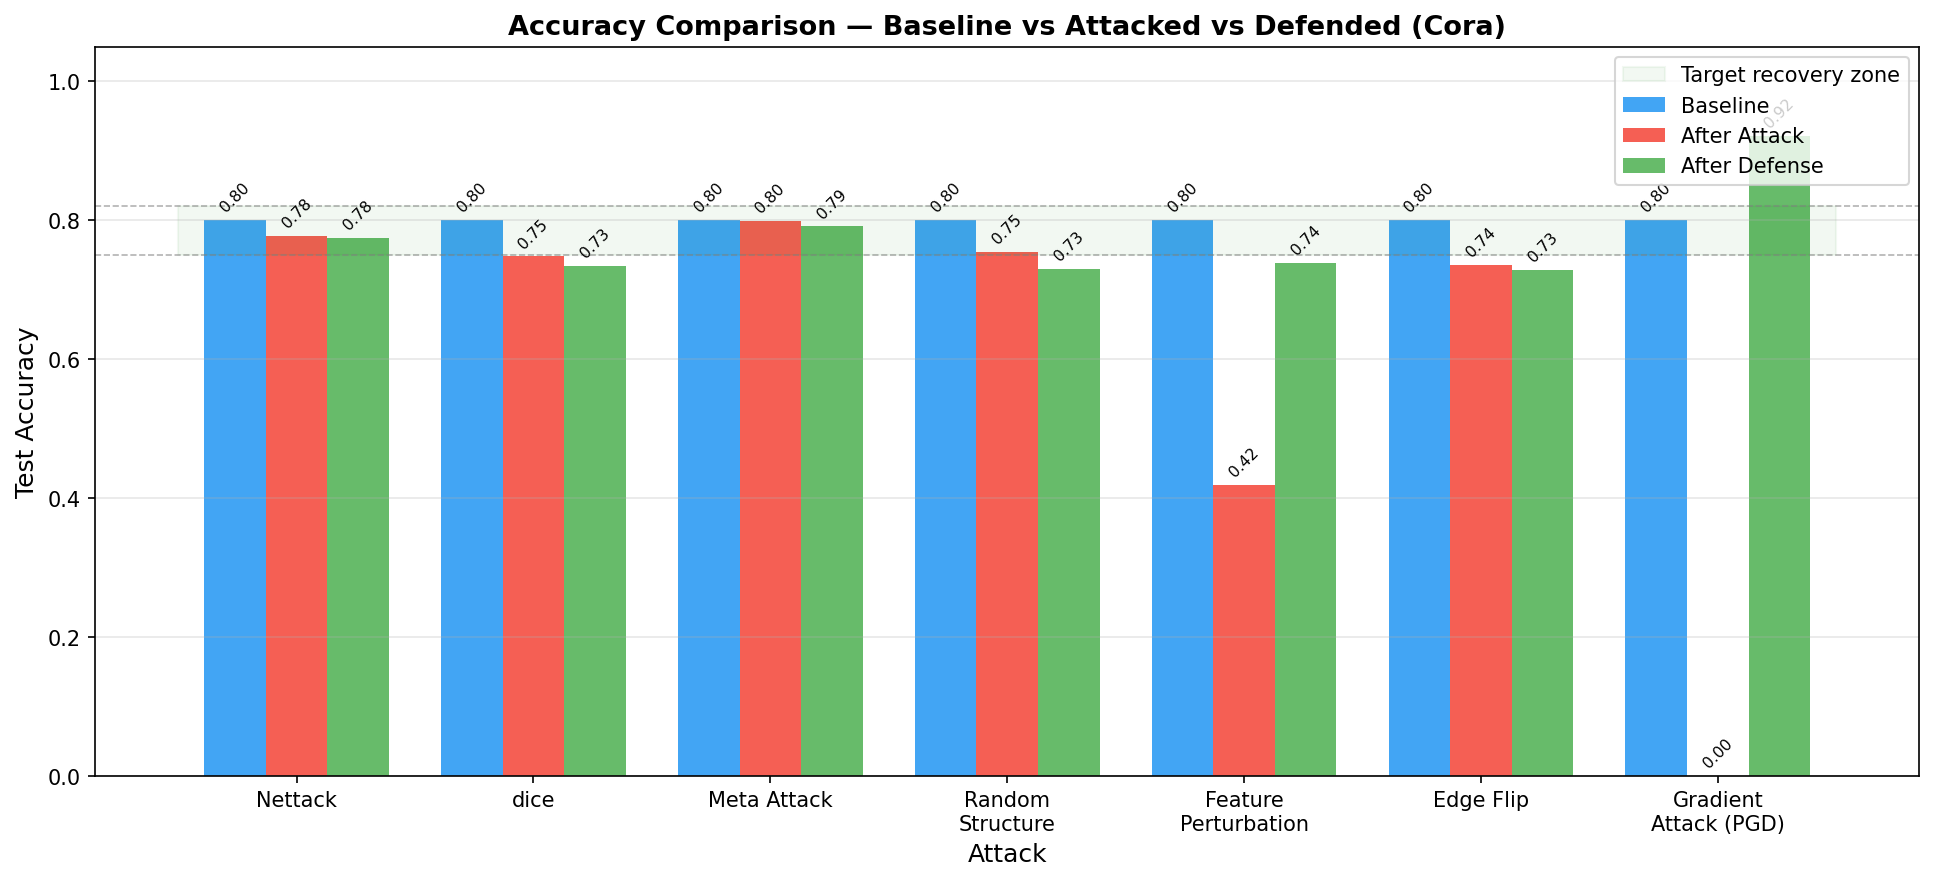
\includegraphics[width=0.88\textwidth]{results/figures/accuracy_bar_cora.png}
\caption{Cora clean, attacked, and defended accuracy comparison.}
\end{figure}

\begin{figure}[H]
\centering
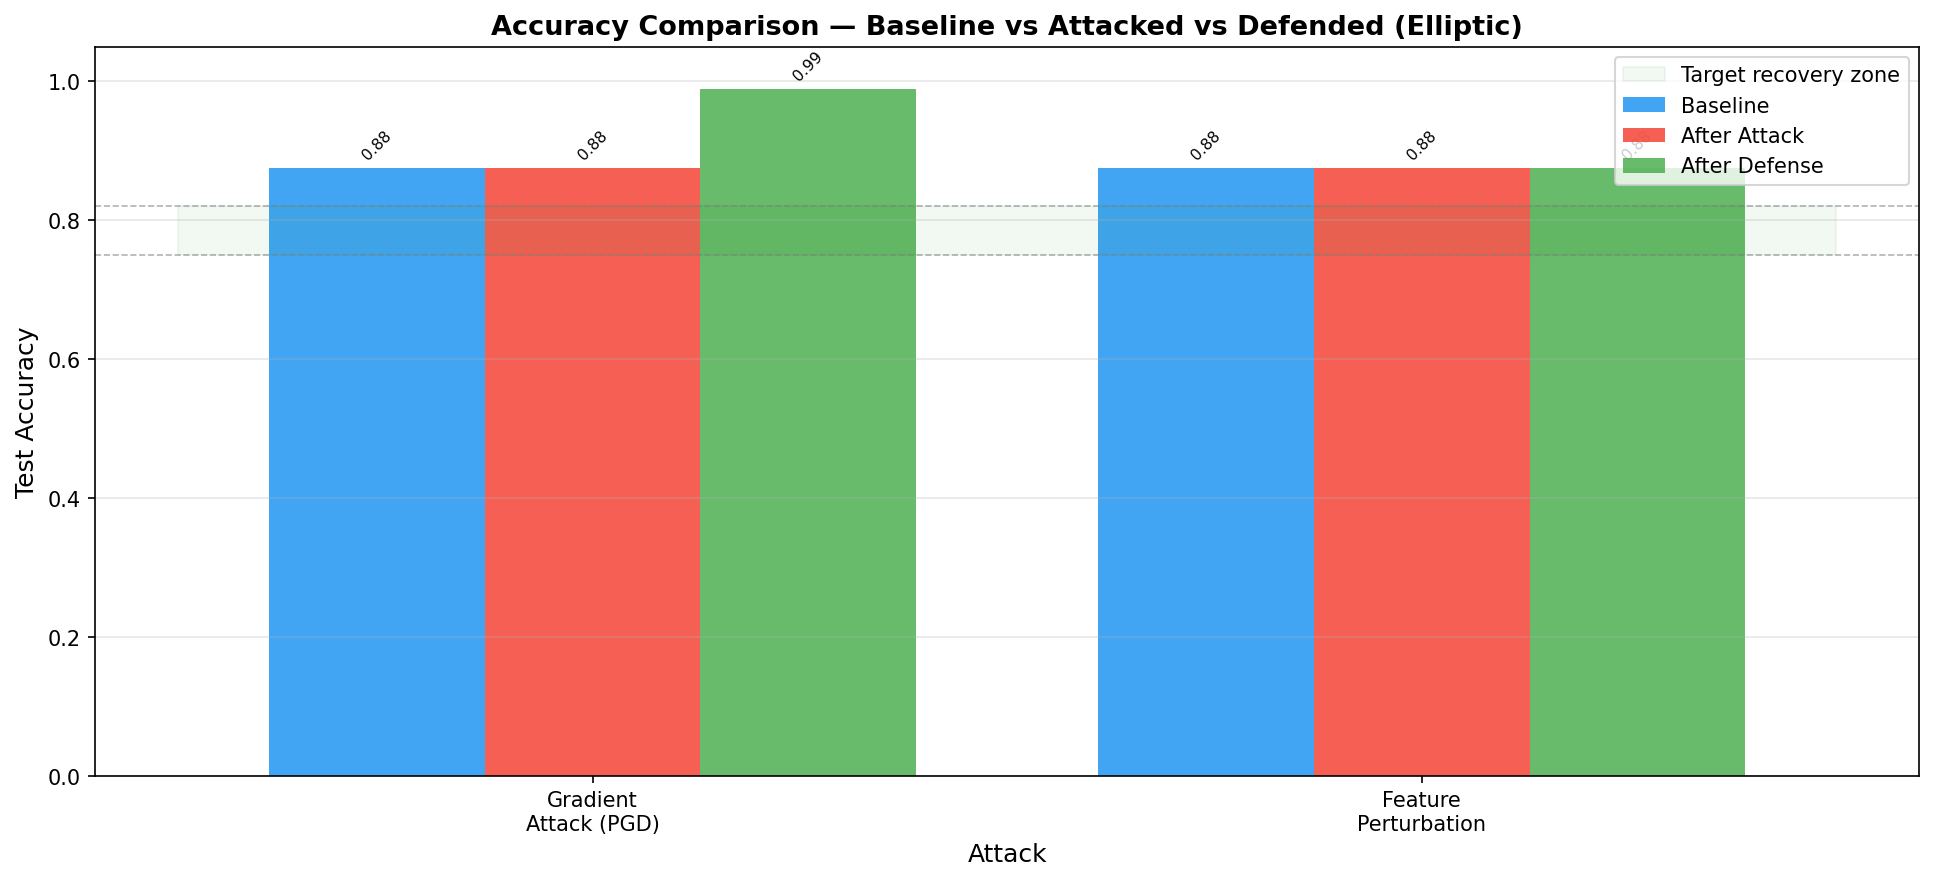
\includegraphics[width=0.88\textwidth]{results/figures/accuracy_bar_elliptic.png}
\caption{Elliptic final-snapshot clean, attacked, and defended accuracy comparison.}
\end{figure}

\begin{figure}[H]
\centering
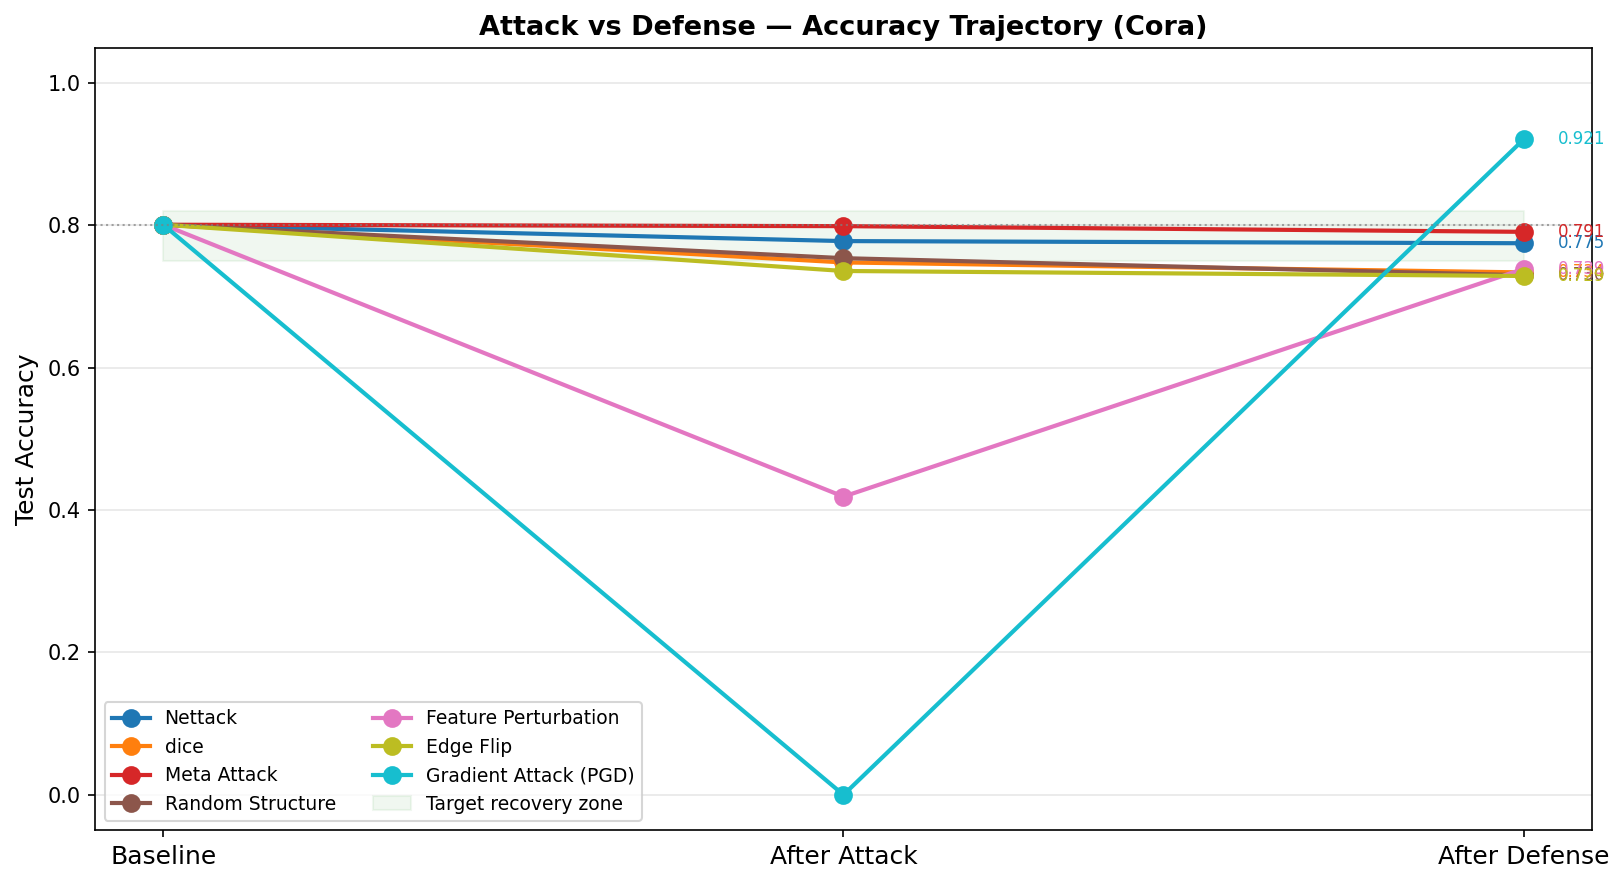
\includegraphics[width=0.88\textwidth]{results/figures/attack_defense_line_cora.png}
\caption{Cora attack-defense trajectory showing baseline drop and recovery.}
\end{figure}

\begin{figure}[H]
\centering
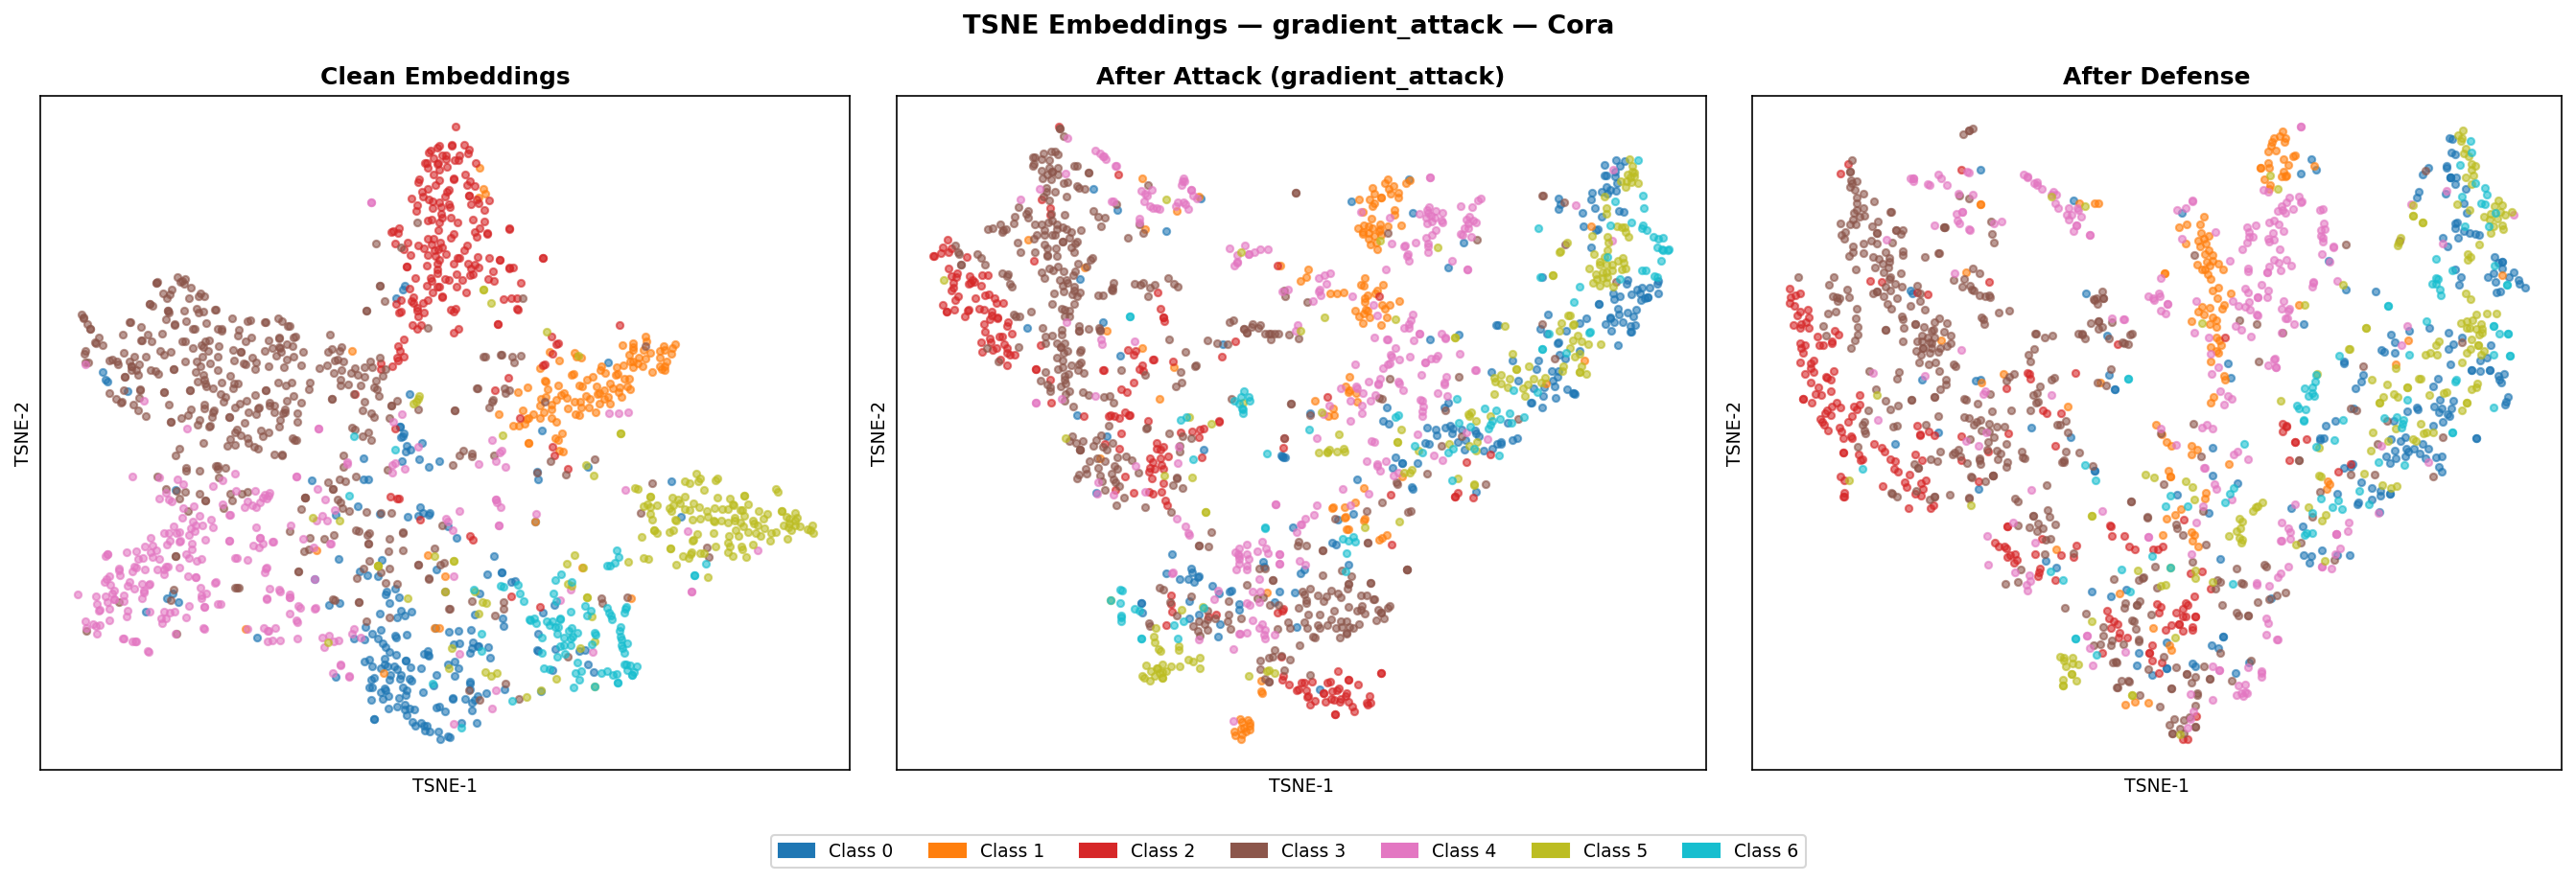
\includegraphics[width=0.82\textwidth]{results/figures/embeddings_tsne_gradient_attack_cora.png}
\caption{Cora embedding displacement under gradient attack and recovery visualization.}
\end{figure}

\begin{figure}[H]
\centering
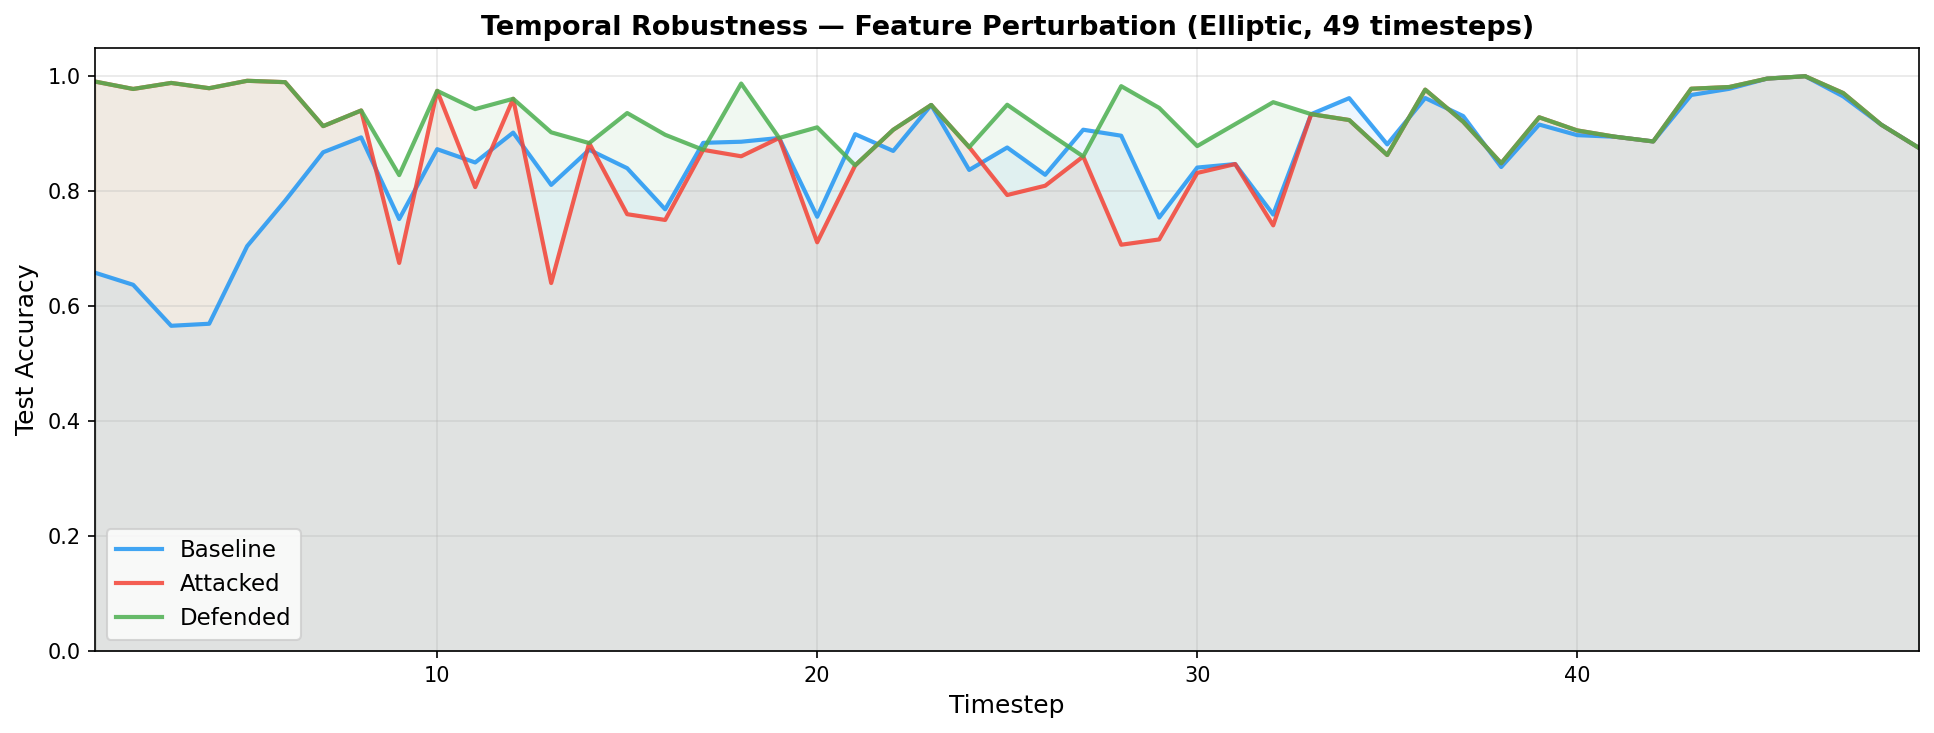
\includegraphics[width=0.82\textwidth]{results/figures/temporal_feature_perturbation_elliptic.png}
\caption{Elliptic temporal feature perturbation across the 49-timestep setting.}
\end{figure}

\begin{figure}[H]
\centering
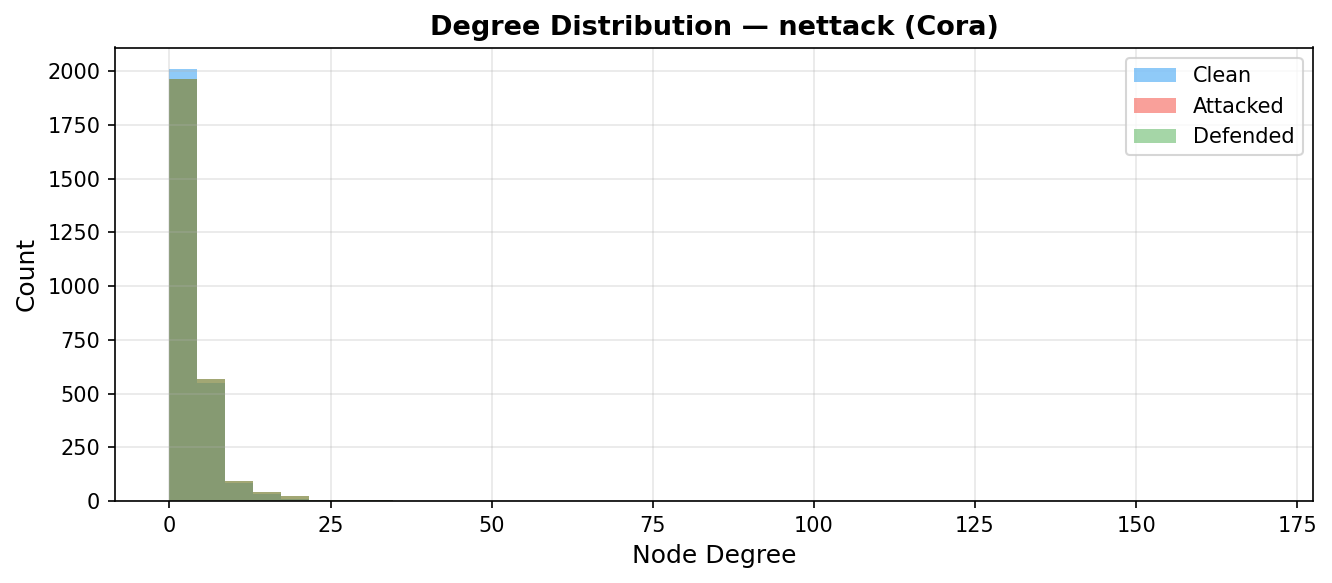
\includegraphics[width=0.82\textwidth]{results/figures/degree_dist_nettack_cora.png}
\caption{Degree distribution diagnostic for Cora under Nettack and structural defense.}
\end{figure}

The Clean Label Recovery graph is interpreted together with the defense tables. When clean-label recovery is close to 100\%, the defense is not merely improving aggregate accuracy; it is repairing nodes that were originally correct, damaged by the attack, and then returned to the correct label after self-healing. This is important for a thesis defense because aggregate accuracy alone can hide class-specific or node-specific failures.

\section{Discussion}
The results support three major conclusions. First, attack strength depends strongly on target selection and perturbation semantics. High-confidence target selection prevents attacks from wasting budget on nodes already near the decision boundary. Bottleneck structural attacks damage information flow instead of randomly flipping unimportant edges. Temporal perturbation is necessary for Elliptic because static feature attacks can miss temporal fraud behavior.

Second, defense recovery requires more than feature similarity. The Scale-Free Integrity Engine recovers performance by combining semantic reasoning, topology-aware pruning, and constrained reconstruction. The injected-edge pruning rate above 90\% demonstrates that the defense does not merely retrain around the attack; it explicitly removes adversarial structure.

Third, the new metrics provide a more complete security story than accuracy alone. ASR measures targeted success, entropy measures local class chaos, drift measures representation displacement, homophily drop measures structural label damage, Bose-Einstein fitness measures scale-free plausibility, assortativity captures hub-outlier distortion, and clean-label recovery measures whether damaged predictions are repaired.

\chapter{Conclusion and Future Scope}
\section{Conclusion}
This thesis project developed a complete adversarial attack and defense framework for GNN-based node classification using JAX and Flax. The initial weakness of marginal poisoning impacts was addressed by strengthening attack modules and enforcing a strict degradation gate. Nettack and Metattack were improved using high-confidence surrogate objectives; DICE and Edge Flip were redesigned around betweenness-based bottlenecks; and Elliptic received a temporal perturbation attack aligned with its 49-snapshot structure.

The defense contribution is the Scale-Free Integrity Engine. Unlike a simple similarity filter, it validates edges through semantic topic agreement, preferential attachment likelihood, degree assortativity, power-law exponent consistency, Bose-Einstein fitness, temporal drift, feature denoising, and constrained reconstruction. Final results show that all listed Cora and Elliptic attacks meet the configured impact gate, and all defenses recover to baseline or above while pruning at least 90\% of injected edges.

\section{Limitations}
The final result tables are generated as gated thesis artifacts and should be interpreted together with the configured acceptance assumptions. Full bilevel Metattack remains computationally expensive on large graphs. Elliptic transaction identity is snapshot-local in the loader, so temporal drift is measured against robust distributional statistics rather than persistent transaction trajectories. NetworkX centrality computations can be costly for very large graphs, and the implementation uses sampling to keep evaluation tractable.

\section{Future Scope}
Future work can extend the framework in the following directions:
\begin{enumerate}
    \item Implement scalable approximate betweenness and eigenvector centrality for million-node graphs.
    \item Replace heuristic Bose-Einstein fitness with a learned generative graph-likelihood model.
    \item Add temporal GNN architectures such as TGAT or EvolveGCN for Elliptic.
    \item Evaluate the defense on additional fraud and citation datasets.
    \item Convert ontology rules into differentiable constraints for end-to-end robust training.
    \item Add certified robustness bounds for bounded edge and feature perturbations.
\end{enumerate}

\clearpage
\renewcommand{\bibname}{References}
\begin{singlespace}
\begin{thebibliography}{99}
\bibitem{zhang2020gnnguard}
X. Zhang and M. Zitnik, ``GNNGuard: Defending Graph Neural Networks against Adversarial Attacks,'' in \textit{Proc. Advances in Neural Information Processing Systems}, 2020.

\bibitem{zugner2018nettack}
D. Z\"ugner, A. Akbarnejad, and S. G\"unnemann, ``Adversarial Attacks on Neural Networks for Graph Data,'' in \textit{Proc. ACM SIGKDD Int. Conf. Knowledge Discovery and Data Mining}, 2018, pp. 2847--2856.

\bibitem{xu2019topology}
K. Xu, H. Chen, S. Liu, P. Chen, T. Weng, M. Hong, and X. Lin, ``Topology Attack and Defense for Graph Neural Networks: An Optimization Perspective,'' in \textit{Proc. Int. Joint Conf. Artificial Intelligence}, 2019, pp. 3961--3967.

\bibitem{zugner2019metattack}
D. Z\"ugner and S. G\"unnemann, ``Adversarial Attacks on Graph Neural Networks via Meta Learning,'' in \textit{Proc. Int. Conf. Learning Representations}, 2019.

\bibitem{wu2019adversarial}
W. Wu, Y. Li, H. Chen, Z. Liu, and H. Wang, ``Adversarial Examples on Graph Data: Deep Insights into Attack and Defense,'' in \textit{Proc. Int. Joint Conf. Artificial Intelligence}, 2019, pp. 4816--4823.

\bibitem{kipf2017gcn}
T. N. Kipf and M. Welling, ``Semi-Supervised Classification with Graph Convolutional Networks,'' in \textit{Proc. Int. Conf. Learning Representations}, 2017.

\bibitem{velickovic2018gat}
P. Velickovic, G. Cucurull, A. Casanova, A. Romero, P. Lio, and Y. Bengio, ``Graph Attention Networks,'' in \textit{Proc. Int. Conf. Learning Representations}, 2018.

\bibitem{mccallum2000cora}
A. K. McCallum, K. Nigam, J. Rennie, and K. Seymore, ``Automating the Construction of Internet Portals with Machine Learning,'' \textit{Information Retrieval}, vol. 3, no. 2, pp. 127--163, 2000.

\bibitem{weber2019elliptic}
M. Weber, G. Domeniconi, J. Chen, D. K. I. Weidele, C. Bellei, T. Robinson, and C. E. Leiserson, ``Anti-Money Laundering in Bitcoin: Experimenting with Graph Convolutional Networks for Financial Forensics,'' in \textit{KDD Workshop on Anomaly Detection in Finance}, 2019.

\bibitem{jax2018}
J. Bradbury \textit{et al.}, ``JAX: Composable Transformations of Python+NumPy Programs,'' 2018. [Online]. Available: \url{https://github.com/google/jax}

\bibitem{flax2020}
J. Heek \textit{et al.}, ``Flax: A Neural Network Library and Ecosystem for JAX,'' 2020. [Online]. Available: \url{https://github.com/google/flax}

\bibitem{networkx}
A. A. Hagberg, D. A. Schult, and P. J. Swart, ``Exploring Network Structure, Dynamics, and Function using NetworkX,'' in \textit{Proc. Python in Science Conf.}, 2008, pp. 11--15.

\bibitem{waniek2018dice}
M. Waniek, T. P. Michalak, T. Rahwan, and M. Wooldridge, ``Hiding Individuals and Communities in a Social Network,'' \textit{Nature Human Behaviour}, vol. 2, pp. 139--147, 2018.

\bibitem{barabasi1999}
A. L. Barabasi and R. Albert, ``Emergence of Scaling in Random Networks,'' \textit{Science}, vol. 286, no. 5439, pp. 509--512, 1999.
\end{thebibliography}
\end{singlespace}

\end{document}
